%! TeX root = master.tex
% !TEX program = lualatex

\lecture{1}{2026-02-16}{}{}

\section{Introduction, Part I}
What happens when you click on a video? How is it possible that a video from the other side of the world appears on my screen? That's what we'll be studying this semester.
\subsection{End-systems, packet switches, links}%
\label{sub:End-systems, packet switches, links}

\textbf{End-system:} All the devices that use internet to communicate (laptop, smarthphone, connected oven, pacemakers, servers streaming/cloud/gaming \ldots).
\\
\textbf{Packet switch:} A network device that enable the end-systems to communicate with one another.
\\
\textbf{Network link:} A physical medium that connects two devices. 

\subsection{Programs, processes, threads}%
\label{sub:Programs, processes, threads}

When invoking a program, the computer creates a new \textbf{process} in the laptop main memory. A process may consist of one or multiple \textbf{threads} (for now only a piece of process). If we invoke multiple times a program, the computer creates multiples processes that are related to that program (one per invocation). See this like an orchestra, the notes = the program, an orchestra playing a piece of music = a process, each instrument = a thread, and they can be multiple ochestra playing at the same time = multiple processes.
\\ \textrightarrow they are the most basic component of the Internet.

\subsection{Distributed Application}%
\label{sub:Distributed Application}
A distributed application, is when different processes that run on potentially different computers and that work toward a common goal.  

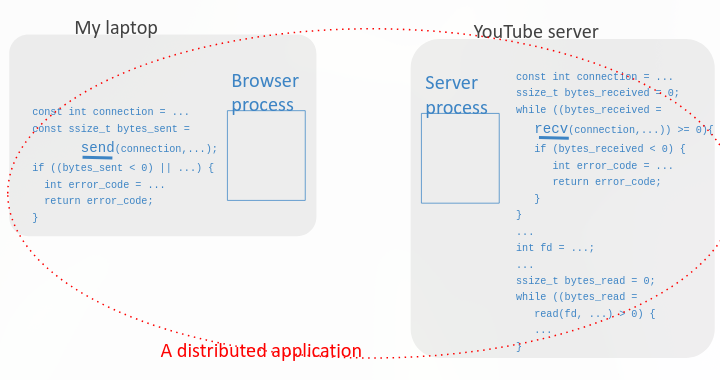
\includegraphics[width=\linewidth]{images/img_20260216_175537.png}
ex: I invoked a browser program on my laptop, which created a browser process in my laptop; some YouTube operator invoked a *server program* on a YouTube server, which created a *server process* in the YouTube server.

\subsection{Communication Protocol}%
\label{sub:Communication Protocol}
\begin{itemize}
\item A specification of \textbf{all possible message sequences} that may be exchanged between the communicating parties.
  \item The \textbf{interface} between the communicating parties. 
  \item It provides an \textbf{abstraction} of the server process (vice versa): one computer can comunicate with other computers without knowing anything about them.
\end{itemize}

\subsection{System calls (syscalls)}%
\label{sub:System calls (syscalls}
\begin{itemize}
  \item Special calls that a process make to access \textbf{computer resources} like storage and network. 
  \item Then \textbf{text} between processes and computer resources.
  \item An \textbf{abstraction} of computer resources presented to processes. 
\end{itemize}
\subsection{Interface & Layers}%
\label{sub:Interface & Layers}

An \textbf{agreement} between two parties about how they will interact. This concept of interfaces inherently create layers.\\ 
\textbf{Layers}:
\begin{itemize}
  \item A collection of entities that conceptuallay play the \textbf{same role}.
  \item Each entity communicates with the \textbf{layer below/above} through a well-defined \textbf{interface}.
\end{itemize}
Interface and layers provide \textbf{abstraction}, which enables \textbf{separation of concerns}. They improve the \textbf{simplicity} and \textbf{flexibiliy}. But, in principle, they do not improve performance.


